\documentclass{standalone}
\usepackage{tikz}
\usetikzlibrary{patterns, positioning}


\begin{document}
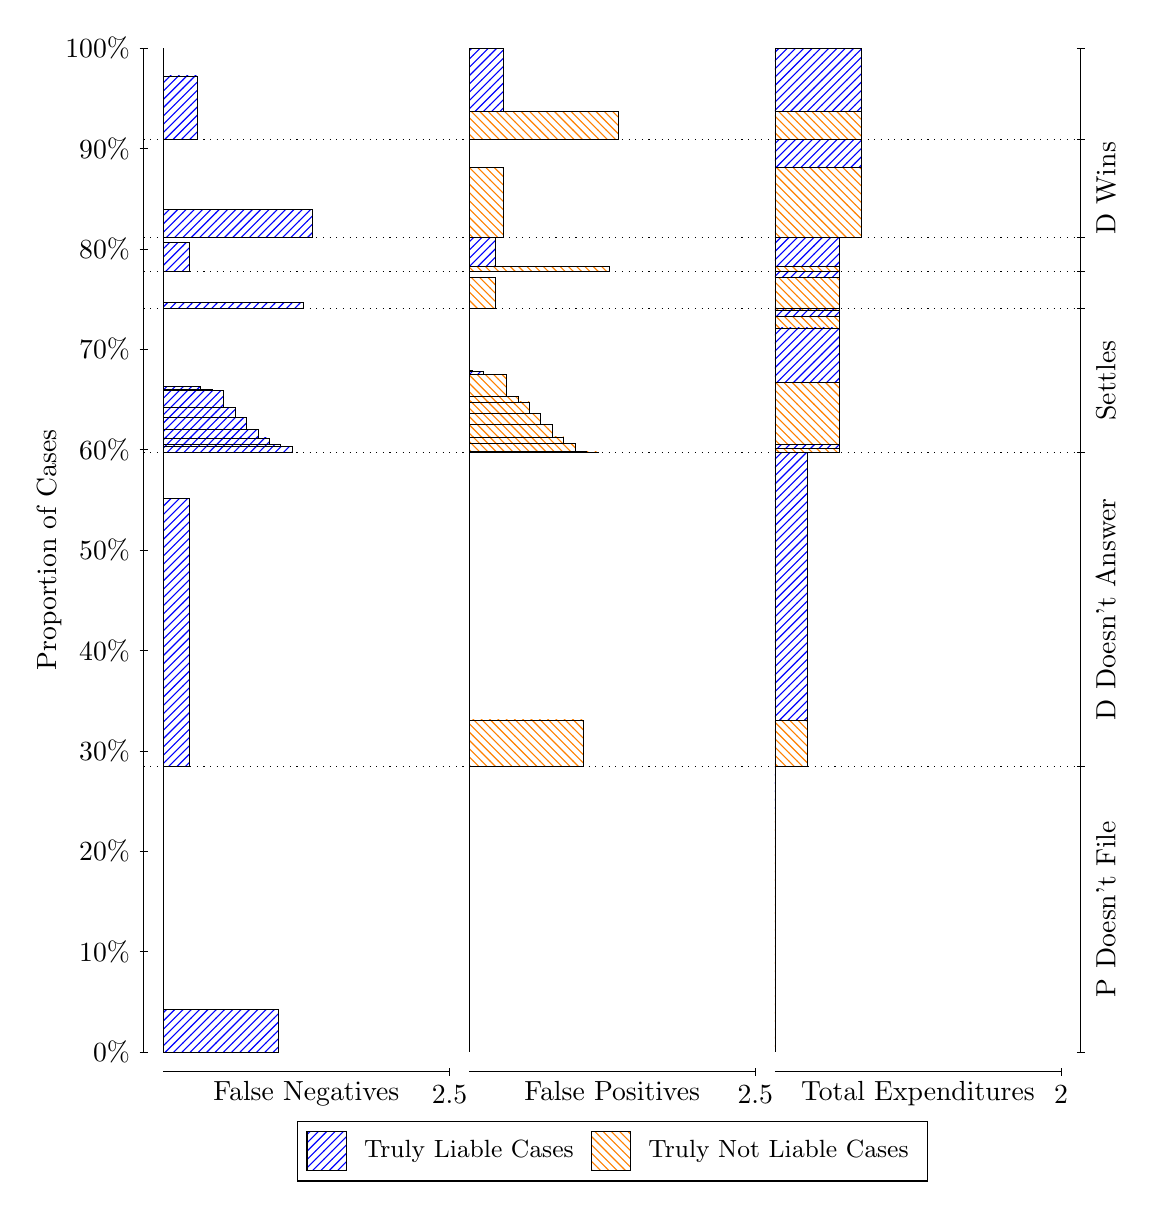
\begin{tikzpicture}
\draw[black, very thin] (1.5,1.75) -- (1.5,14.5);
\node[rotate=90, text=black, anchor=center] at (0.3, 8.125) {Proportion of Cases};
\draw[black, very thin] (1.45,1.75) -- (1.55,1.75);
\node[text=black, anchor=east] at (1.45, 1.75) {0\%};
\draw[black, very thin] (1.45,3.025) -- (1.55,3.025);
\node[text=black, anchor=east] at (1.45, 3.025) {10\%};
\draw[black, very thin] (1.45,4.3) -- (1.55,4.3);
\node[text=black, anchor=east] at (1.45, 4.3) {20\%};
\draw[black, very thin] (1.45,5.575) -- (1.55,5.575);
\node[text=black, anchor=east] at (1.45, 5.575) {30\%};
\draw[black, very thin] (1.45,6.85) -- (1.55,6.85);
\node[text=black, anchor=east] at (1.45, 6.85) {40\%};
\draw[black, very thin] (1.45,8.125) -- (1.55,8.125);
\node[text=black, anchor=east] at (1.45, 8.125) {50\%};
\draw[black, very thin] (1.45,9.4) -- (1.55,9.4);
\node[text=black, anchor=east] at (1.45, 9.4) {60\%};
\draw[black, very thin] (1.45,10.675) -- (1.55,10.675);
\node[text=black, anchor=east] at (1.45, 10.675) {70\%};
\draw[black, very thin] (1.45,11.95) -- (1.55,11.95);
\node[text=black, anchor=east] at (1.45, 11.95) {80\%};
\draw[black, very thin] (1.45,13.225) -- (1.55,13.225);
\node[text=black, anchor=east] at (1.45, 13.225) {90\%};
\draw[black, very thin] (1.45,14.5) -- (1.55,14.5);
\node[text=black, anchor=east] at (1.45, 14.5) {100\%};

\draw[black, very thin] (13.4,1.75) -- (13.4,14.5);
\draw[black, very thin] (13.35,1.75) -- (13.45,1.75);
\node[anchor=west] at (13.35, 1.75) {};
\draw[black, very thin] (13.35,5.3782) -- (13.45,5.3782);
\node[anchor=west] at (13.35, 5.3782) {};
\draw[black, very thin] (13.35,9.3659) -- (13.45,9.3659);
\node[anchor=west] at (13.35, 9.3659) {};
\draw[black, very thin] (13.35,11.191) -- (13.45,11.191);
\node[anchor=west] at (13.35, 11.191) {};
\draw[black, very thin] (13.35,11.664) -- (13.45,11.664);
\node[anchor=west] at (13.35, 11.664) {};
\draw[black, very thin] (13.35,12.095) -- (13.45,12.095);
\node[anchor=west] at (13.35, 12.095) {};
\draw[black, very thin] (13.35,13.34) -- (13.45,13.34);
\node[anchor=west] at (13.35, 13.34) {};
\draw[black, very thin] (13.35,14.5) -- (13.45,14.5);
\node[anchor=west] at (13.35, 14.5) {};

\draw[black, very thin, pattern color=blue, pattern=north east lines] (1.75,1.75) rectangle (3.2033,2.2894);
\draw[black, very thin, pattern color=orange, pattern=north west lines] (1.75,2.2894) rectangle (1.75,5.3782);
\draw[black, very thin, pattern color=blue, pattern=north east lines] (1.75,5.3782) rectangle (2.077,8.7775);
\draw[black, very thin, pattern color=orange, pattern=north west lines] (1.75,8.7775) rectangle (1.75,9.3659);
\draw[black, very thin, pattern color=blue, pattern=north east lines] (1.75,9.3659) rectangle (3.385,9.4421);
\draw[black, very thin, pattern color=blue, pattern=north east lines] (1.75,9.4421) rectangle (3.2397,9.4697);
\draw[black, very thin, pattern color=blue, pattern=north east lines] (1.75,9.4697) rectangle (3.0943,9.5475);
\draw[black, very thin, pattern color=blue, pattern=north east lines] (1.75,9.5475) rectangle (2.949,9.6522);
\draw[black, very thin, pattern color=blue, pattern=north east lines] (1.75,9.6522) rectangle (2.8037,9.8131);
\draw[black, very thin, pattern color=blue, pattern=north east lines] (1.75,9.8131) rectangle (2.6583,9.9358);
\draw[black, very thin, pattern color=blue, pattern=north east lines] (1.75,9.9358) rectangle (2.513,10.151);
\draw[black, very thin, pattern color=blue, pattern=north east lines] (1.75,10.151) rectangle (2.3677,10.168);
\draw[black, very thin, pattern color=blue, pattern=north east lines] (1.75,10.168) rectangle (2.2223,10.2);
\draw[black, very thin, pattern color=orange, pattern=north west lines] (1.75,10.2) rectangle (1.75,11.191);
\draw[black, very thin, pattern color=blue, pattern=north east lines] (1.75,11.191) rectangle (3.5303,11.265);
\draw[black, very thin, pattern color=orange, pattern=north west lines] (1.75,11.265) rectangle (1.75,11.664);
\draw[black, very thin, pattern color=blue, pattern=north east lines] (1.75,11.664) rectangle (2.077,12.031);
\draw[black, very thin, pattern color=orange, pattern=north west lines] (1.75,12.031) rectangle (1.75,12.095);
\draw[black, very thin, pattern color=blue, pattern=north east lines] (1.75,12.095) rectangle (3.6393,12.449);
\draw[black, very thin, pattern color=orange, pattern=north west lines] (1.75,12.449) rectangle (1.75,13.34);
\draw[black, very thin, pattern color=blue, pattern=north east lines] (1.75,13.34) rectangle (2.186,14.147);
\draw[black, very thin, pattern color=orange, pattern=north west lines] (1.75,14.147) rectangle (1.75,14.5);
\draw[black, very thin, pattern color=orange, pattern=north west lines] (5.6333,1.75) rectangle (5.6333,4.8388);
\draw[black, very thin, pattern color=blue, pattern=north east lines] (5.6333,4.8388) rectangle (5.6333,5.3782);
\draw[black, very thin, pattern color=orange, pattern=north west lines] (5.6333,5.3782) rectangle (7.0867,5.9665);
\draw[black, very thin, pattern color=blue, pattern=north east lines] (5.6333,5.9665) rectangle (5.6333,9.3659);
\draw[black, very thin, pattern color=orange, pattern=north west lines] (5.6333,9.3659) rectangle (7.2683,9.3706);
\draw[black, very thin, pattern color=orange, pattern=north west lines] (5.6333,9.3706) rectangle (7.123,9.3749);
\draw[black, very thin, pattern color=orange, pattern=north west lines] (5.6333,9.3749) rectangle (6.9777,9.4756);
\draw[black, very thin, pattern color=orange, pattern=north west lines] (5.6333,9.4756) rectangle (6.8323,9.5605);
\draw[black, very thin, pattern color=orange, pattern=north west lines] (5.6333,9.5605) rectangle (6.687,9.7232);
\draw[black, very thin, pattern color=orange, pattern=north west lines] (5.6333,9.7232) rectangle (6.5417,9.8602);
\draw[black, very thin, pattern color=orange, pattern=north west lines] (5.6333,9.8602) rectangle (6.3963,10.007);
\draw[black, very thin, pattern color=orange, pattern=north west lines] (5.6333,10.007) rectangle (6.251,10.071);
\draw[black, very thin, pattern color=orange, pattern=north west lines] (5.6333,10.071) rectangle (6.1057,10.357);
\draw[black, very thin, pattern color=blue, pattern=north east lines] (5.6333,10.357) rectangle (5.815,10.389);
\draw[black, very thin, pattern color=blue, pattern=north east lines] (5.6333,10.389) rectangle (5.6697,10.406);
\draw[black, very thin, pattern color=blue, pattern=north east lines] (5.6333,10.406) rectangle (5.6333,11.191);
\draw[black, very thin, pattern color=orange, pattern=north west lines] (5.6333,11.191) rectangle (5.9603,11.59);
\draw[black, very thin, pattern color=blue, pattern=north east lines] (5.6333,11.59) rectangle (5.6333,11.664);
\draw[black, very thin, pattern color=orange, pattern=north west lines] (5.6333,11.664) rectangle (7.4137,11.728);
\draw[black, very thin, pattern color=blue, pattern=north east lines] (5.6333,11.728) rectangle (5.9603,12.095);
\draw[black, very thin, pattern color=orange, pattern=north west lines] (5.6333,12.095) rectangle (6.0693,12.986);
\draw[black, very thin, pattern color=blue, pattern=north east lines] (5.6333,12.986) rectangle (5.6333,13.34);
\draw[black, very thin, pattern color=orange, pattern=north west lines] (5.6333,13.34) rectangle (7.5227,13.693);
\draw[black, very thin, pattern color=blue, pattern=north east lines] (5.6333,13.693) rectangle (6.0693,14.5);
\draw[black, very thin, pattern color=orange, pattern=north west lines] (9.5167,1.75) rectangle (9.5167,4.8388);
\draw[black, very thin, pattern color=blue, pattern=north east lines] (9.5167,4.8388) rectangle (9.5167,5.3782);
\draw[black, very thin, pattern color=orange, pattern=north west lines] (9.5167,5.3782) rectangle (9.9254,5.9665);
\draw[black, very thin, pattern color=blue, pattern=north east lines] (9.5167,5.9665) rectangle (9.9254,9.3659);
\draw[black, very thin, pattern color=orange, pattern=north west lines] (9.5167,9.3659) rectangle (10.334,9.4196);
\draw[black, very thin, pattern color=blue, pattern=north east lines] (9.5167,9.4196) rectangle (10.334,9.469);
\draw[black, very thin, pattern color=orange, pattern=north west lines] (9.5167,9.469) rectangle (10.334,10.255);
\draw[black, very thin, pattern color=blue, pattern=north east lines] (9.5167,10.255) rectangle (10.334,10.945);
\draw[black, very thin, pattern color=orange, pattern=north west lines] (9.5167,10.945) rectangle (10.334,11.092);
\draw[black, very thin, pattern color=blue, pattern=north east lines] (9.5167,11.092) rectangle (10.334,11.17);
\draw[black, very thin, pattern color=orange, pattern=north west lines] (9.5167,11.17) rectangle (10.334,11.174);
\draw[black, very thin, pattern color=blue, pattern=north east lines] (9.5167,11.174) rectangle (10.334,11.191);
\draw[black, very thin, pattern color=orange, pattern=north west lines] (9.5167,11.191) rectangle (10.334,11.59);
\draw[black, very thin, pattern color=blue, pattern=north east lines] (9.5167,11.59) rectangle (10.334,11.664);
\draw[black, very thin, pattern color=orange, pattern=north west lines] (9.5167,11.664) rectangle (10.334,11.728);
\draw[black, very thin, pattern color=blue, pattern=north east lines] (9.5167,11.728) rectangle (10.334,12.095);
\draw[black, very thin, pattern color=orange, pattern=north west lines] (9.5167,12.095) rectangle (10.607,12.986);
\draw[black, very thin, pattern color=blue, pattern=north east lines] (9.5167,12.986) rectangle (10.607,13.34);
\draw[black, very thin, pattern color=orange, pattern=north west lines] (9.5167,13.34) rectangle (10.607,13.693);
\draw[black, very thin, pattern color=blue, pattern=north east lines] (9.5167,13.693) rectangle (10.607,14.5);
\draw[black, dotted] (1.5,5.3782) -- (13.4,5.3782);
\draw[black, dotted] (1.5,9.3659) -- (13.4,9.3659);
\draw[black, dotted] (1.5,11.191) -- (13.4,11.191);
\draw[black, dotted] (1.5,11.664) -- (13.4,11.664);
\draw[black, dotted] (1.5,12.095) -- (13.4,12.095);
\draw[black, dotted] (1.5,13.34) -- (13.4,13.34);
\draw[black, very thin] (1.75,1.5) -- (5.3833,1.5);
\node[text=black, anchor=north] at (3.5667, 1.5) {False Negatives};
\draw[black, very thin] (5.3833,1.45) -- (5.3833,1.55);
\node[text=black, anchor=north] at (5.3833, 1.45) {2.5};

\draw[black, very thin] (5.6333,1.5) -- (9.2667,1.5);
\node[text=black, anchor=north] at (7.45, 1.5) {False Positives};
\draw[black, very thin] (9.2667,1.45) -- (9.2667,1.55);
\node[text=black, anchor=north] at (9.2667, 1.45) {2.5};

\draw[black, very thin] (9.5167,1.5) -- (13.15,1.5);
\node[text=black, anchor=north] at (11.333, 1.5) {Total Expenditures};
\draw[black, very thin] (13.15,1.45) -- (13.15,1.55);
\node[text=black, anchor=north] at (13.15, 1.45) {2};

\node[text=black, centered, rotate=90] at (13.72, 3.5641) {P Doesn't File};
\node[text=black, centered, rotate=90] at (13.72, 7.372) {D Doesn't Answer};
\node[text=black, centered, rotate=90] at (13.72, 10.279) {Settles};


\node[text=black, centered, rotate=90] at (13.72, 12.717) {D Wins};


\draw (7.449999999999999,1.5) node[draw=none] (baseCoordinate) {};
\begin{scope}[align=center]
        \matrix[scale=0.5, draw=black, below=0.5cm of baseCoordinate, nodes={draw}, column sep=0.1cm]{
            \node[rectangle, draw, minimum width=0.5cm, minimum height=0.5cm, pattern color=blue, pattern=north east lines] {}; &
            \node[draw=none, font=\small, text=black] (B) {Truly Liable Cases}; &
            \node[rectangle, draw, minimum width=0.5cm, minimum height=0.5cm, pattern color=orange, pattern=north west lines] {}; &
            \node[draw=none, font=\small, text=black] (B) {Truly Not Liable Cases}; \\
            };
\end{scope}

\end{tikzpicture}
\end{document}